\documentclass[12pt,-letter paper]{article}
\usepackage{siunitx}
\usepackage{setspace}
\usepackage{gensymb}
\usepackage{xcolor}
\usepackage{caption}
%\usepackage{subcaption}
\doublespacing
\singlespacing
\usepackage[none]{hyphenat}
\usepackage{amssymb}
\usepackage{relsize}
\usepackage[cmex10]{amsmath}
\usepackage{mathtools}
\usepackage{amsmath}
\usepackage{commath}
\usepackage{amsthm}
\interdisplaylinepenalty=2500
%\savesymbol{iint}
\usepackage{txfonts}
%\restoresymbol{TXF}{iint}
\usepackage{wasysym}
\usepackage{amsthm}
\usepackage{mathrsfs}
\usepackage{txfonts}
\let\vec\mathbf{}
\usepackage{stfloats}
\usepackage{float}
\usepackage{cite}
\usepackage{cases}
\usepackage{subfig}
%\usepackage{xtab}
\usepackage{longtable}
\usepackage{multirow}
%\usepackage{algorithm}
\usepackage{amssymb}
%\usepackage{algpseudocode}
\usepackage{enumitem}
\usepackage{mathtools}
%\usepackage{eenrc}
%\usepackage[framemethod=tikz]{mdframed}
\usepackage{listings}
%\usepackage{listings}
\usepackage[latin1]{inputenc}
%%\usepackage{color}{   
%%\usepackage{lscape}
\usepackage{textcomp}
\usepackage{titling}
\usepackage{hyperref}
%\usepackage{fulbigskip}   
\usepackage{tikz}
\usepackage{graphicx}
\lstset{
  frame=single,
  breaklines=true
}
\let\vec\mathbf{}
\usepackage{enumitem}
\usepackage{graphicx}
\usepackage{siunitx}
\let\vec\mathbf{}
\usepackage{enumitem}
\usepackage{graphicx}
\usepackage{enumitem}
\usepackage{tfrupee}
\usepackage{amsmath}
\usepackage{amssymb}
\usepackage{mwe} % for blindtext and example-image-a in example
\usepackage{wrapfig}
\graphicspath{{figs/}}
\providecommand{\mydet}[1]{\ensuremath{\begin{vmatrix}#1\end{\vmatrix}}}
\providecommand{\myvec}[1]{\ensuremath{\begin{bmatrix}#1\end{\bmatrix}}}
\providecommand{\cbrak}[1]{\ensuremath{\left\{#1\right\}}}
\providecommand{\brak}[1]{\ensuremath{\left(#1\right)}}
\begin {document}
\section {Relations} 
\begin {enumerate}
\item \begin {enumerate}
\item [(a)] Students of a school are taken to a railway museum to learn about railway heritage and its history.
        \begin {figure} [h!]
        \centering
        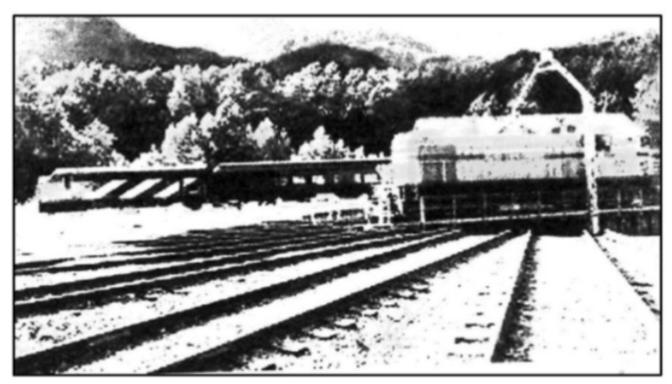
\includegraphics[width=0.8\textwidth] {/storage/emulated/0/DCIM/Screenshots/figure1.jpg}
        \end {figure}                                                                                                                                     
\\ An exhibit in the museum depicted many rail lines on the track near the railway station. Let $L$ be the set of all rail lines on the railway track and $R$ be the relation on $L$ defined by
\begin {align*}
R=\cbrak{\brak{l_1,l_2}: l_1 \parallel l_2}
\end {align*}
On the basis of the above information, answer the following questions:

\begin {enumerate}
\item [(i)] Find whether the relation $R$ is symmetric or not.
\item [(ii)] Find whether the relation $R$ is transitive or not.
\item [(iii)] If one of the rail lines on the  railway track is represented by the equation $y=3x+2$, then find the set of rail lines in $R$ related to it.
\end {enumerate}
\item [(b)] Let $S$ be the relation defined by 
	S=\cbrak{\brak{l_1, l_2}:l_1 \perp l_2} check whether the relation $S$ is symmetric and transitive.
\end {enumerate}
\end {enumerate}
\end {document}
~
